\documentclass{standalone}
\usepackage{tikz}
\usetikzlibrary{patterns, positioning}


\begin{document}
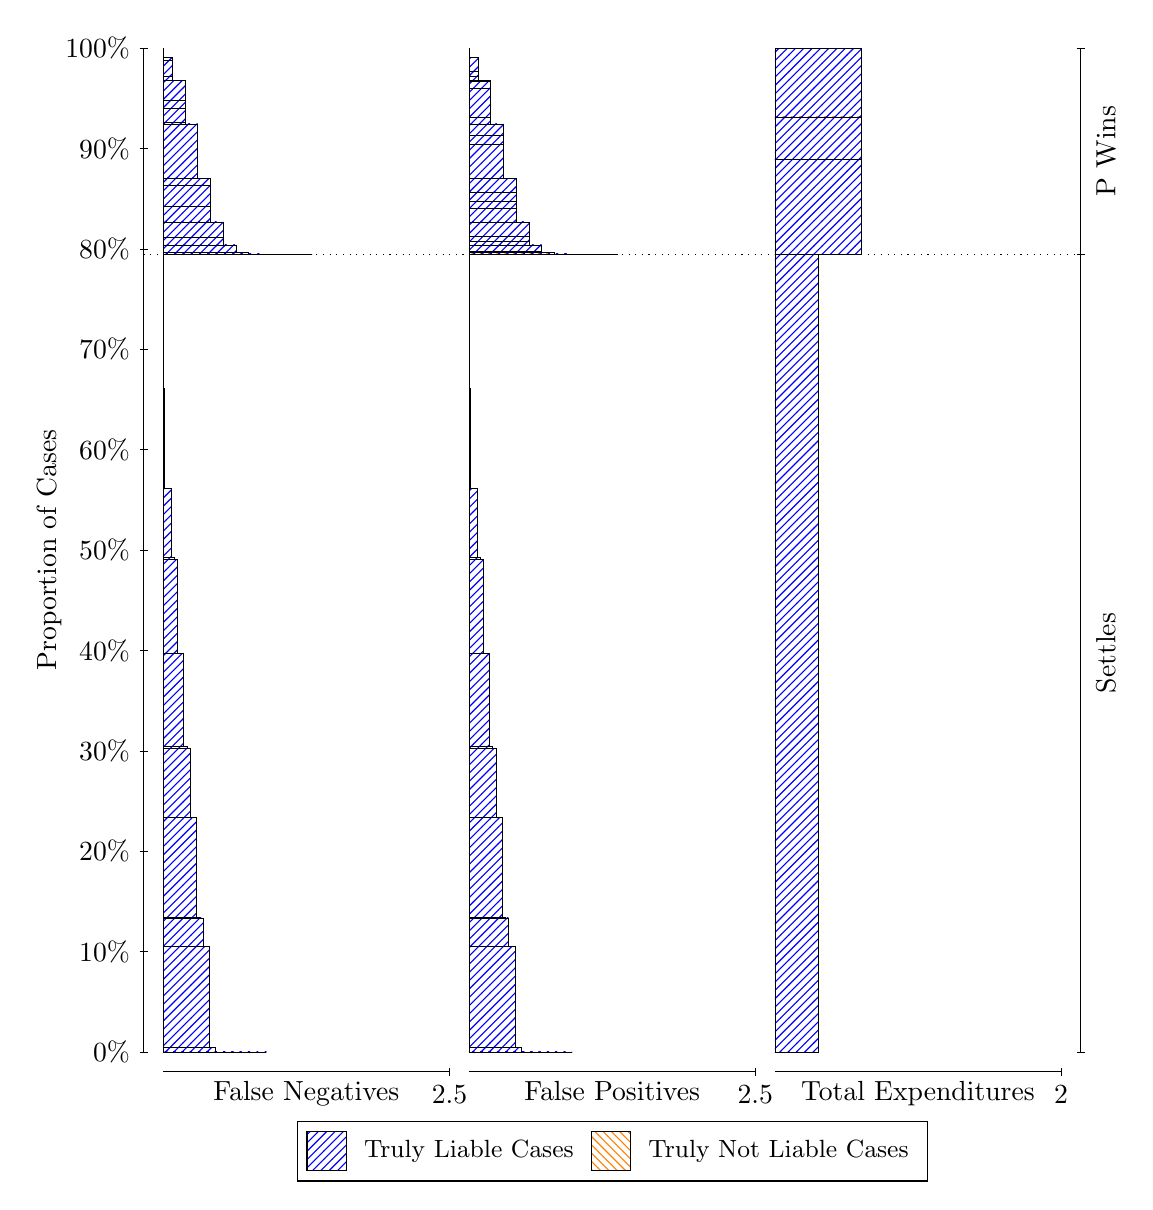
\begin{tikzpicture}
\draw[black, very thin] (1.5,1.75) -- (1.5,14.5);
\node[rotate=90, text=black, anchor=center] at (0.3, 8.125) {Proportion of Cases};
\draw[black, very thin] (1.45,1.75) -- (1.55,1.75);
\node[text=black, anchor=east] at (1.45, 1.75) {0\%};
\draw[black, very thin] (1.45,3.025) -- (1.55,3.025);
\node[text=black, anchor=east] at (1.45, 3.025) {10\%};
\draw[black, very thin] (1.45,4.3) -- (1.55,4.3);
\node[text=black, anchor=east] at (1.45, 4.3) {20\%};
\draw[black, very thin] (1.45,5.575) -- (1.55,5.575);
\node[text=black, anchor=east] at (1.45, 5.575) {30\%};
\draw[black, very thin] (1.45,6.85) -- (1.55,6.85);
\node[text=black, anchor=east] at (1.45, 6.85) {40\%};
\draw[black, very thin] (1.45,8.125) -- (1.55,8.125);
\node[text=black, anchor=east] at (1.45, 8.125) {50\%};
\draw[black, very thin] (1.45,9.4) -- (1.55,9.4);
\node[text=black, anchor=east] at (1.45, 9.4) {60\%};
\draw[black, very thin] (1.45,10.675) -- (1.55,10.675);
\node[text=black, anchor=east] at (1.45, 10.675) {70\%};
\draw[black, very thin] (1.45,11.95) -- (1.55,11.95);
\node[text=black, anchor=east] at (1.45, 11.95) {80\%};
\draw[black, very thin] (1.45,13.225) -- (1.55,13.225);
\node[text=black, anchor=east] at (1.45, 13.225) {90\%};
\draw[black, very thin] (1.45,14.5) -- (1.55,14.5);
\node[text=black, anchor=east] at (1.45, 14.5) {100\%};

\draw[black, very thin] (13.4,1.75) -- (13.4,14.5);
\draw[black, very thin] (13.35,1.75) -- (13.45,1.75);
\node[anchor=west] at (13.35, 1.75) {};
\draw[black, very thin] (13.35,11.883) -- (13.45,11.883);
\node[anchor=west] at (13.35, 11.883) {};
\draw[black, very thin] (13.35,14.5) -- (13.45,14.5);
\node[anchor=west] at (13.35, 14.5) {};

\draw[black, very thin, pattern color=blue, pattern=north east lines] (1.75,1.75) rectangle (3.058,1.75);
\draw[black, very thin, pattern color=blue, pattern=north east lines] (1.75,1.75) rectangle (2.8965,1.75);
\draw[black, very thin, pattern color=blue, pattern=north east lines] (1.75,1.75) rectangle (2.735,1.75);
\draw[black, very thin, pattern color=blue, pattern=north east lines] (1.75,1.75) rectangle (2.6947,1.75);
\draw[black, very thin, pattern color=blue, pattern=north east lines] (1.75,1.75) rectangle (2.5736,1.7525);
\draw[black, very thin, pattern color=blue, pattern=north east lines] (1.75,1.7525) rectangle (2.5332,1.7525);
\draw[black, very thin, pattern color=blue, pattern=north east lines] (1.75,1.7525) rectangle (2.4121,1.8114);
\draw[black, very thin, pattern color=blue, pattern=north east lines] (1.75,1.8114) rectangle (2.3717,1.8117);
\draw[black, very thin, pattern color=blue, pattern=north east lines] (1.75,1.8117) rectangle (2.3313,3.0862);
\draw[black, very thin, pattern color=blue, pattern=north east lines] (1.75,3.0862) rectangle (2.2506,3.4534);
\draw[black, very thin, pattern color=blue, pattern=north east lines] (1.75,3.4534) rectangle (2.2102,3.4588);
\draw[black, very thin, pattern color=blue, pattern=north east lines] (1.75,3.4588) rectangle (2.1699,4.7254);
\draw[black, very thin, pattern color=blue, pattern=north east lines] (1.75,4.7254) rectangle (2.0891,5.6014);
\draw[black, very thin, pattern color=blue, pattern=north east lines] (1.75,5.6014) rectangle (2.0487,5.6277);
\draw[black, very thin, pattern color=blue, pattern=north east lines] (1.75,5.6277) rectangle (2.0084,6.8167);
\draw[black, very thin, pattern color=blue, pattern=north east lines] (1.75,6.8167) rectangle (1.9276,8.0057);
\draw[black, very thin, pattern color=blue, pattern=north east lines] (1.75,8.0057) rectangle (1.8873,8.032);
\draw[black, very thin, pattern color=blue, pattern=north east lines] (1.75,8.032) rectangle (1.8469,8.9081);
\draw[black, very thin, pattern color=blue, pattern=north east lines] (1.75,8.9081) rectangle (1.7661,10.175);
\draw[black, very thin, pattern color=orange, pattern=north west lines] (1.75,10.175) rectangle (1.75,10.175);
\draw[black, very thin, pattern color=blue, pattern=north east lines] (1.75,10.175) rectangle (1.75,11.883);
\draw[black, very thin, pattern color=blue, pattern=north east lines] (1.75,11.883) rectangle (3.6393,11.883);
\draw[black, very thin, pattern color=blue, pattern=north east lines] (1.75,11.883) rectangle (3.4779,11.883);
\draw[black, very thin, pattern color=blue, pattern=north east lines] (1.75,11.883) rectangle (3.3164,11.883);
\draw[black, very thin, pattern color=blue, pattern=north east lines] (1.75,11.883) rectangle (3.1549,11.883);
\draw[black, very thin, pattern color=blue, pattern=north east lines] (1.75,11.883) rectangle (3.1549,11.883);
\draw[black, very thin, pattern color=blue, pattern=north east lines] (1.75,11.883) rectangle (2.9934,11.885);
\draw[black, very thin, pattern color=blue, pattern=north east lines] (1.75,11.885) rectangle (2.9934,11.885);
\draw[black, very thin, pattern color=blue, pattern=north east lines] (1.75,11.885) rectangle (2.8319,11.903);
\draw[black, very thin, pattern color=blue, pattern=north east lines] (1.75,11.903) rectangle (2.6704,12);
\draw[black, very thin, pattern color=blue, pattern=north east lines] (1.75,12) rectangle (2.509,12.091);
\draw[black, very thin, pattern color=blue, pattern=north east lines] (1.75,12.091) rectangle (2.509,12.291);
\draw[black, very thin, pattern color=blue, pattern=north east lines] (1.75,12.291) rectangle (2.3475,12.291);
\draw[black, very thin, pattern color=blue, pattern=north east lines] (1.75,12.291) rectangle (2.3475,12.484);
\draw[black, very thin, pattern color=blue, pattern=north east lines] (1.75,12.484) rectangle (2.3475,12.762);
\draw[black, very thin, pattern color=blue, pattern=north east lines] (1.75,12.762) rectangle (2.3475,12.847);
\draw[black, very thin, pattern color=blue, pattern=north east lines] (1.75,12.847) rectangle (2.186,12.85);
\draw[black, very thin, pattern color=blue, pattern=north east lines] (1.75,12.85) rectangle (2.186,13.536);
\draw[black, very thin, pattern color=blue, pattern=north east lines] (1.75,13.536) rectangle (2.0245,13.555);
\draw[black, very thin, pattern color=blue, pattern=north east lines] (1.75,13.555) rectangle (2.0245,13.729);
\draw[black, very thin, pattern color=blue, pattern=north east lines] (1.75,13.729) rectangle (2.0245,13.835);
\draw[black, very thin, pattern color=blue, pattern=north east lines] (1.75,13.835) rectangle (2.0245,14.092);
\draw[black, very thin, pattern color=blue, pattern=north east lines] (1.75,14.092) rectangle (1.863,14.146);
\draw[black, very thin, pattern color=blue, pattern=north east lines] (1.75,14.146) rectangle (1.863,14.34);
\draw[black, very thin, pattern color=blue, pattern=north east lines] (1.75,14.34) rectangle (1.863,14.384);
\draw[black, very thin, pattern color=orange, pattern=north west lines] (1.75,14.384) rectangle (1.75,14.384);
\draw[black, very thin, pattern color=blue, pattern=north east lines] (1.75,14.384) rectangle (1.75,14.5);
\draw[black, very thin, pattern color=orange, pattern=north west lines] (5.6333,1.75) rectangle (6.9413,1.75);
\draw[black, very thin, pattern color=blue, pattern=north east lines] (5.6333,1.75) rectangle (6.9413,1.75);
\draw[black, very thin, pattern color=blue, pattern=north east lines] (5.6333,1.75) rectangle (6.7799,1.75);
\draw[black, very thin, pattern color=blue, pattern=north east lines] (5.6333,1.75) rectangle (6.6184,1.75);
\draw[black, very thin, pattern color=orange, pattern=north west lines] (5.6333,1.75) rectangle (6.578,1.75);
\draw[black, very thin, pattern color=blue, pattern=north east lines] (5.6333,1.75) rectangle (6.578,1.75);
\draw[black, very thin, pattern color=blue, pattern=north east lines] (5.6333,1.75) rectangle (6.4569,1.7525);
\draw[black, very thin, pattern color=blue, pattern=north east lines] (5.6333,1.7525) rectangle (6.4165,1.7525);
\draw[black, very thin, pattern color=blue, pattern=north east lines] (5.6333,1.7525) rectangle (6.2954,1.8114);
\draw[black, very thin, pattern color=blue, pattern=north east lines] (5.6333,1.8114) rectangle (6.255,1.8116);
\draw[black, very thin, pattern color=orange, pattern=north west lines] (5.6333,1.8116) rectangle (6.2147,1.8116);
\draw[black, very thin, pattern color=blue, pattern=north east lines] (5.6333,1.8116) rectangle (6.2147,3.0862);
\draw[black, very thin, pattern color=blue, pattern=north east lines] (5.6333,3.0862) rectangle (6.1339,3.4533);
\draw[black, very thin, pattern color=blue, pattern=north east lines] (5.6333,3.4533) rectangle (6.0936,3.4588);
\draw[black, very thin, pattern color=blue, pattern=north east lines] (5.6333,3.4588) rectangle (6.0532,4.7253);
\draw[black, very thin, pattern color=blue, pattern=north east lines] (5.6333,4.7253) rectangle (5.9724,5.6013);
\draw[black, very thin, pattern color=blue, pattern=north east lines] (5.6333,5.6013) rectangle (5.9321,5.6276);
\draw[black, very thin, pattern color=blue, pattern=north east lines] (5.6333,5.6276) rectangle (5.8917,6.8166);
\draw[black, very thin, pattern color=blue, pattern=north east lines] (5.6333,6.8166) rectangle (5.811,8.0056);
\draw[black, very thin, pattern color=blue, pattern=north east lines] (5.6333,8.0056) rectangle (5.7706,8.0319);
\draw[black, very thin, pattern color=blue, pattern=north east lines] (5.6333,8.0319) rectangle (5.7302,8.908);
\draw[black, very thin, pattern color=blue, pattern=north east lines] (5.6333,8.908) rectangle (5.6495,10.175);
\draw[black, very thin, pattern color=blue, pattern=north east lines] (5.6333,10.175) rectangle (5.6333,11.883);
\draw[black, very thin, pattern color=orange, pattern=north west lines] (5.6333,11.883) rectangle (7.5227,11.883);
\draw[black, very thin, pattern color=blue, pattern=north east lines] (5.6333,11.883) rectangle (7.5227,11.883);
\draw[black, very thin, pattern color=orange, pattern=north west lines] (5.6333,11.883) rectangle (7.3612,11.883);
\draw[black, very thin, pattern color=blue, pattern=north east lines] (5.6333,11.883) rectangle (7.3612,11.883);
\draw[black, very thin, pattern color=blue, pattern=north east lines] (5.6333,11.883) rectangle (7.1997,11.883);
\draw[black, very thin, pattern color=orange, pattern=north west lines] (5.6333,11.883) rectangle (7.1997,11.883);
\draw[black, very thin, pattern color=blue, pattern=north east lines] (5.6333,11.883) rectangle (7.1997,11.883);
\draw[black, very thin, pattern color=blue, pattern=north east lines] (5.6333,11.883) rectangle (7.0382,11.883);
\draw[black, very thin, pattern color=blue, pattern=north east lines] (5.6333,11.883) rectangle (7.0382,11.883);
\draw[black, very thin, pattern color=orange, pattern=north west lines] (5.6333,11.883) rectangle (7.0382,11.883);
\draw[black, very thin, pattern color=blue, pattern=north east lines] (5.6333,11.883) rectangle (7.0382,11.883);
\draw[black, very thin, pattern color=orange, pattern=north west lines] (5.6333,11.883) rectangle (6.8767,11.883);
\draw[black, very thin, pattern color=blue, pattern=north east lines] (5.6333,11.883) rectangle (6.8767,11.885);
\draw[black, very thin, pattern color=blue, pattern=north east lines] (5.6333,11.885) rectangle (6.8767,11.885);
\draw[black, very thin, pattern color=blue, pattern=north east lines] (5.6333,11.885) rectangle (6.8767,11.885);
\draw[black, very thin, pattern color=orange, pattern=north west lines] (5.6333,11.885) rectangle (6.7153,11.885);
\draw[black, very thin, pattern color=blue, pattern=north east lines] (5.6333,11.885) rectangle (6.7153,11.902);
\draw[black, very thin, pattern color=blue, pattern=north east lines] (5.6333,11.902) rectangle (6.7153,11.903);
\draw[black, very thin, pattern color=blue, pattern=north east lines] (5.6333,11.903) rectangle (6.5538,11.922);
\draw[black, very thin, pattern color=orange, pattern=north west lines] (5.6333,11.922) rectangle (6.5538,11.922);
\draw[black, very thin, pattern color=blue, pattern=north east lines] (5.6333,11.922) rectangle (6.5538,12);
\draw[black, very thin, pattern color=blue, pattern=north east lines] (5.6333,12) rectangle (6.3923,12.043);
\draw[black, very thin, pattern color=blue, pattern=north east lines] (5.6333,12.043) rectangle (6.3923,12.107);
\draw[black, very thin, pattern color=orange, pattern=north west lines] (5.6333,12.107) rectangle (6.3923,12.107);
\draw[black, very thin, pattern color=blue, pattern=north east lines] (5.6333,12.107) rectangle (6.3923,12.291);
\draw[black, very thin, pattern color=blue, pattern=north east lines] (5.6333,12.291) rectangle (6.2308,12.467);
\draw[black, very thin, pattern color=blue, pattern=north east lines] (5.6333,12.467) rectangle (6.2308,12.55);
\draw[black, very thin, pattern color=orange, pattern=north west lines] (5.6333,12.55) rectangle (6.2308,12.55);
\draw[black, very thin, pattern color=blue, pattern=north east lines] (5.6333,12.55) rectangle (6.2308,12.671);
\draw[black, very thin, pattern color=blue, pattern=north east lines] (5.6333,12.671) rectangle (6.2308,12.673);
\draw[black, very thin, pattern color=blue, pattern=north east lines] (5.6333,12.673) rectangle (6.2308,12.847);
\draw[black, very thin, pattern color=blue, pattern=north east lines] (5.6333,12.847) rectangle (6.0693,13.28);
\draw[black, very thin, pattern color=orange, pattern=north west lines] (5.6333,13.28) rectangle (6.0693,13.28);
\draw[black, very thin, pattern color=blue, pattern=north east lines] (5.6333,13.28) rectangle (6.0693,13.386);
\draw[black, very thin, pattern color=blue, pattern=north east lines] (5.6333,13.386) rectangle (6.0693,13.536);
\draw[black, very thin, pattern color=blue, pattern=north east lines] (5.6333,13.536) rectangle (5.9079,13.619);
\draw[black, very thin, pattern color=blue, pattern=north east lines] (5.6333,13.619) rectangle (5.9079,13.99);
\draw[black, very thin, pattern color=blue, pattern=north east lines] (5.6333,13.99) rectangle (5.9079,14.073);
\draw[black, very thin, pattern color=blue, pattern=north east lines] (5.6333,14.073) rectangle (5.9079,14.092);
\draw[black, very thin, pattern color=blue, pattern=north east lines] (5.6333,14.092) rectangle (5.7464,14.146);
\draw[black, very thin, pattern color=blue, pattern=north east lines] (5.6333,14.146) rectangle (5.7464,14.2);
\draw[black, very thin, pattern color=blue, pattern=north east lines] (5.6333,14.2) rectangle (5.7464,14.384);
\draw[black, very thin, pattern color=blue, pattern=north east lines] (5.6333,14.384) rectangle (5.6333,14.5);
\draw[black, very thin, pattern color=orange, pattern=north west lines] (9.5167,1.75) rectangle (10.062,1.75);
\draw[black, very thin, pattern color=blue, pattern=north east lines] (9.5167,1.75) rectangle (10.062,11.883);
\draw[black, very thin, pattern color=orange, pattern=north west lines] (9.5167,11.883) rectangle (10.607,11.883);
\draw[black, very thin, pattern color=blue, pattern=north east lines] (9.5167,11.883) rectangle (10.607,13.082);
\draw[black, very thin, pattern color=orange, pattern=north west lines] (9.5167,13.082) rectangle (10.607,13.082);
\draw[black, very thin, pattern color=blue, pattern=north east lines] (9.5167,13.082) rectangle (10.607,13.626);
\draw[black, very thin, pattern color=orange, pattern=north west lines] (9.5167,13.626) rectangle (10.607,13.626);
\draw[black, very thin, pattern color=blue, pattern=north east lines] (9.5167,13.626) rectangle (10.607,14.5);
\draw[black, dotted] (1.5,11.883) -- (13.4,11.883);
\draw[black, very thin] (1.75,1.5) -- (5.3833,1.5);
\node[text=black, anchor=north] at (3.5667, 1.5) {False Negatives};
\draw[black, very thin] (5.3833,1.45) -- (5.3833,1.55);
\node[text=black, anchor=north] at (5.3833, 1.45) {2.5};

\draw[black, very thin] (5.6333,1.5) -- (9.2667,1.5);
\node[text=black, anchor=north] at (7.45, 1.5) {False Positives};
\draw[black, very thin] (9.2667,1.45) -- (9.2667,1.55);
\node[text=black, anchor=north] at (9.2667, 1.45) {2.5};

\draw[black, very thin] (9.5167,1.5) -- (13.15,1.5);
\node[text=black, anchor=north] at (11.333, 1.5) {Total Expenditures};
\draw[black, very thin] (13.15,1.45) -- (13.15,1.55);
\node[text=black, anchor=north] at (13.15, 1.45) {2};

\node[text=black, centered, rotate=90] at (13.72, 6.8167) {Settles};
\node[text=black, centered, rotate=90] at (13.72, 13.192) {P Wins};

\draw (7.449999999999999,1.5) node[draw=none] (baseCoordinate) {};
\begin{scope}[align=center]
        \matrix[scale=0.5, draw=black, below=0.5cm of baseCoordinate, nodes={draw}, column sep=0.1cm]{
            \node[rectangle, draw, minimum width=0.5cm, minimum height=0.5cm, pattern color=blue, pattern=north east lines] {}; &
            \node[draw=none, font=\small, text=black] (B) {Truly Liable Cases}; &
            \node[rectangle, draw, minimum width=0.5cm, minimum height=0.5cm, pattern color=orange, pattern=north west lines] {}; &
            \node[draw=none, font=\small, text=black] (B) {Truly Not Liable Cases}; \\
            };
\end{scope}

\end{tikzpicture}
\end{document}